\section{Linear Regression}
\noindent
{\color{LightRubineRed} \rule{\linewidth}{1mm} }
\subsection{Linear Regression hypothesis}
\begin{align*}
h(x) = W^Tx
\end{align*}
\begin{myremark}{Importance}
Find \textcolor{mypink2}{lines/hyperplanes} with small \textcolor{mypink3}{residuals}.
\end{myremark}
\textbf{The Error Measure}
\begin{align*}
E_{in}(w) &= \frac{1}{N}\sum_{n=1}^N  (w^Tx_n - y_n)^2 \\
E_{out}(h) &= \underset{x \sim P}{\mathbb{E}} (w^Tx_n - y_n)^2\\
\end{align*}
\textbf{Min $E_{in}$ ?} 
\subsection{Linear Regression Algorithm}
\begin{align*}
E_{in}(w) &= \frac{1}{N}\sum_{n=1}^N  (w^Tx_n - y_n)^2 \\
          &= \frac{1}{N} {||XW -Y||}^2
\end{align*}
\begin{align*}
\; let \ \nabla_{w}E = 0 \\
E_{in}(W) &= \frac{1}{N} {||XW -Y||}^2 \\
       &= \frac{1}{N} (W^T\underbrace{X^TX}_AW - W^T\underbrace{X^Ty}_b + \underbrace{y^Ty}_c) \\
       &= \frac{1}{N}(W^TAW - 2W^Tb + c) \\
\nabla_{W}E &= \frac{1}{N}(2AW-2b) \\
            &= \frac{2}{N}(AW-b) \\
            &= 0 \\
W^* = \underbrace{(X^TX)^{-1}X^T}_{pseudo-inverse}y
\end{align*}
\subsection{Generalization issue}
不像是一个学习的过程,而是一步登天。 \par
不是特别懂呀。。 \par

\subsection{Linear Classification vs. Linear Regression}
\begin{center}
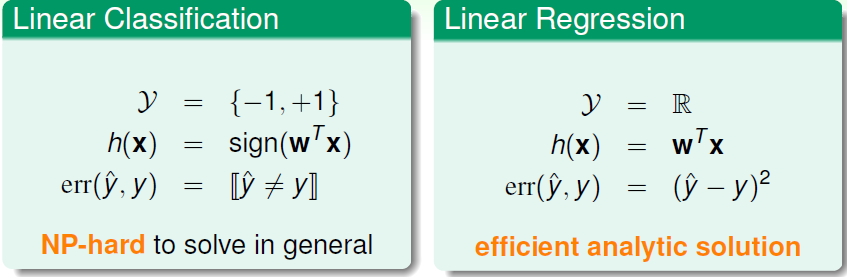
\includegraphics[width=10cm, height=4cm]{lecture9_1}\\
\end{center}
可以用LR来优化linear Classification。VC 理论可以保证学习。 \par
\begin{center}
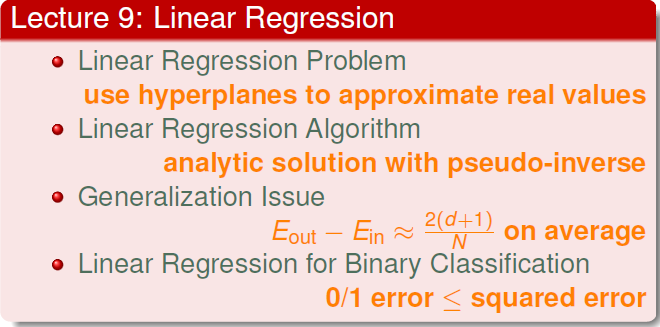
\includegraphics[width=8cm, height=5cm]{lecture9_sum}\\
\end{center}

\noindent
{\color{RubineRed} \rule{\linewidth}{1mm} }